\subsection{Comparison of heuristics and techniques}\label{app:comparison}
\Cref{fig:comparison} shows the effect of our heuristics and optimizations for
aligning complex short sequences. The effect of pruning is most noticeable for
\CSH and \GCH without DT. \GCH is our most accurate heuristic, so, as expected,
it leads to the lowest number of expanded states.

\begin{figure*}[t]
  \centering
  \begin{tabular}{l>{\centering}m{0.18\linewidth}>{\centering}m{0.18\linewidth}>{\centering}m{0.18\linewidth}>{\centering\arraybackslash}m{0.35\linewidth}}
    & \textbf{Base} & \textbf{Pruning} & \textbf{DT} & \textbf{Pruning + DT} \\
    \textbf{Dijkstra} &
    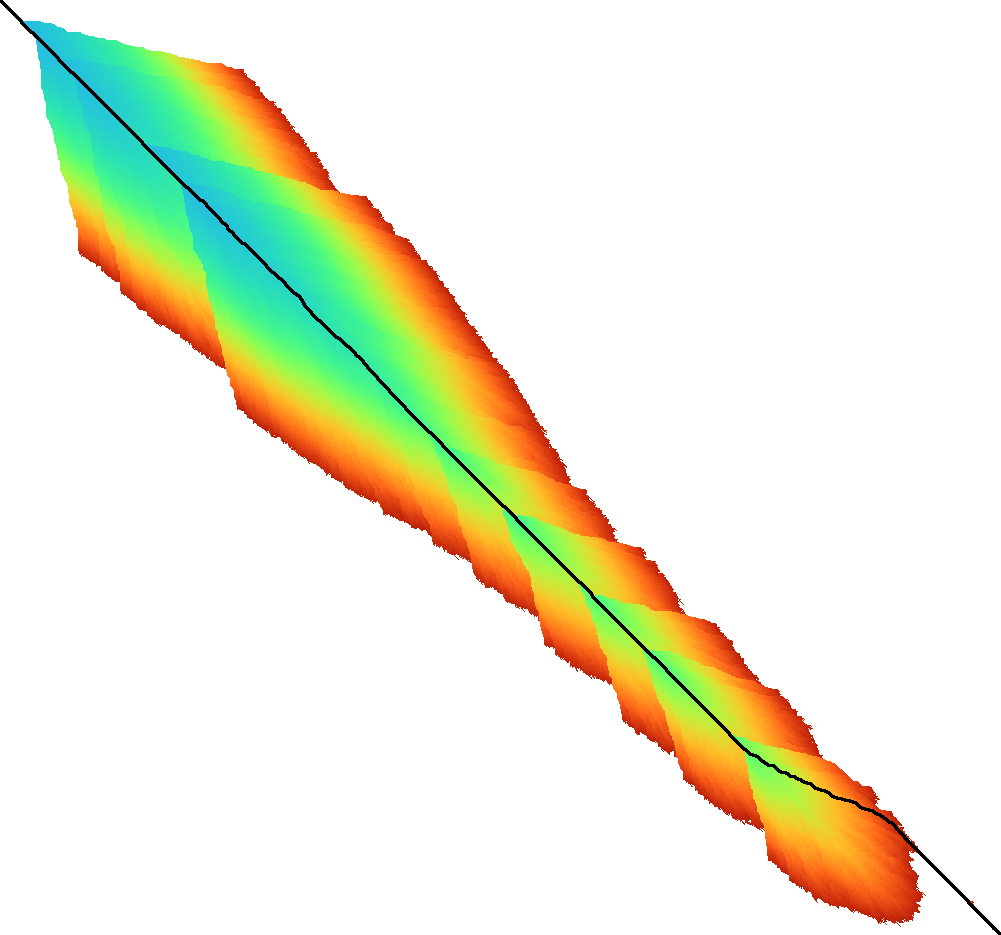
\includegraphics[scale=0.15]{imgs/comparison/dijkstra-noprune.png} &
    &
    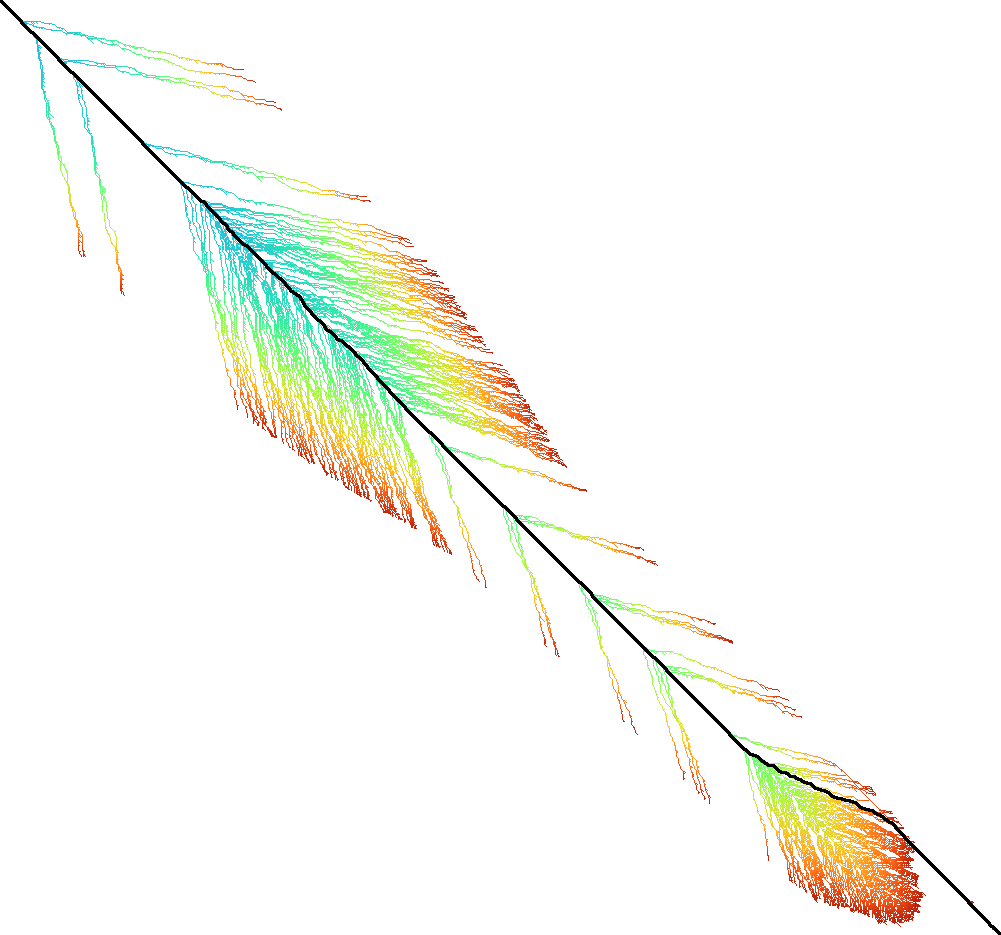
\includegraphics[scale=0.15]{imgs/comparison/dijkstra-noprune-dt.png} &
    \\[1cm]
    \textbf{SH} &
    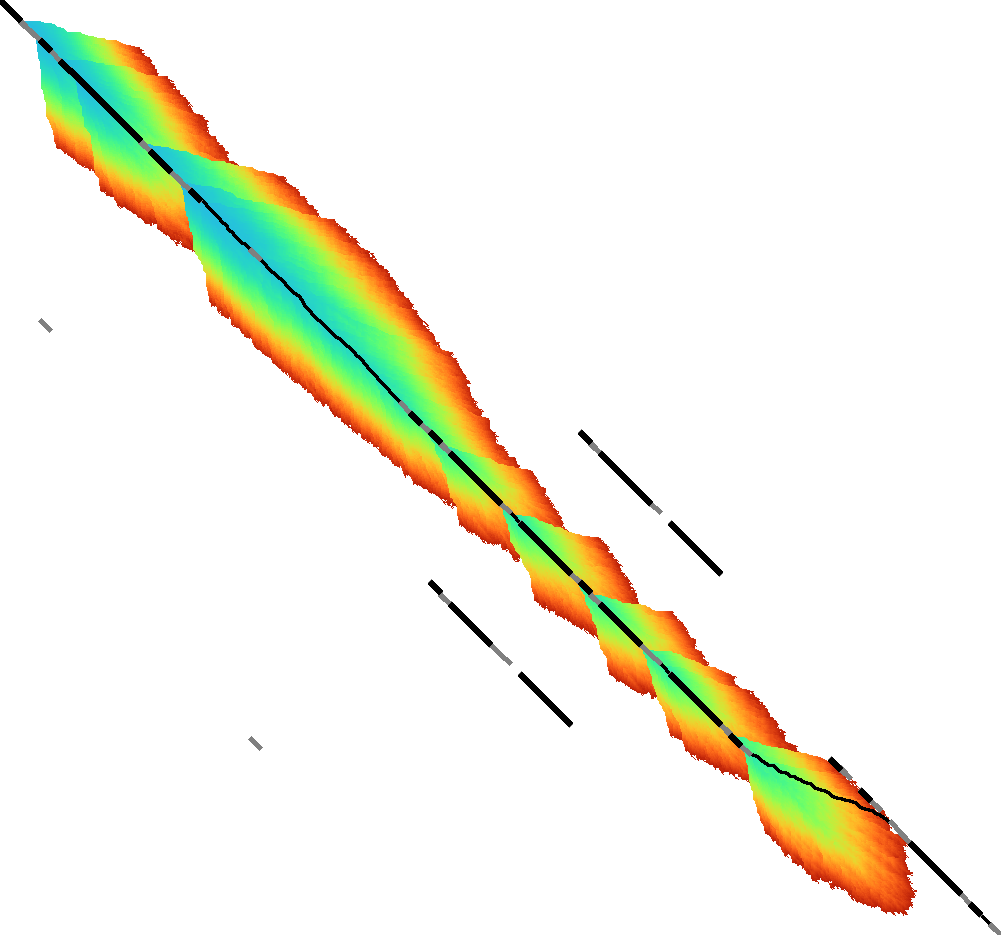
\includegraphics[scale=0.15]{imgs/comparison/sh-noprune.png} &
    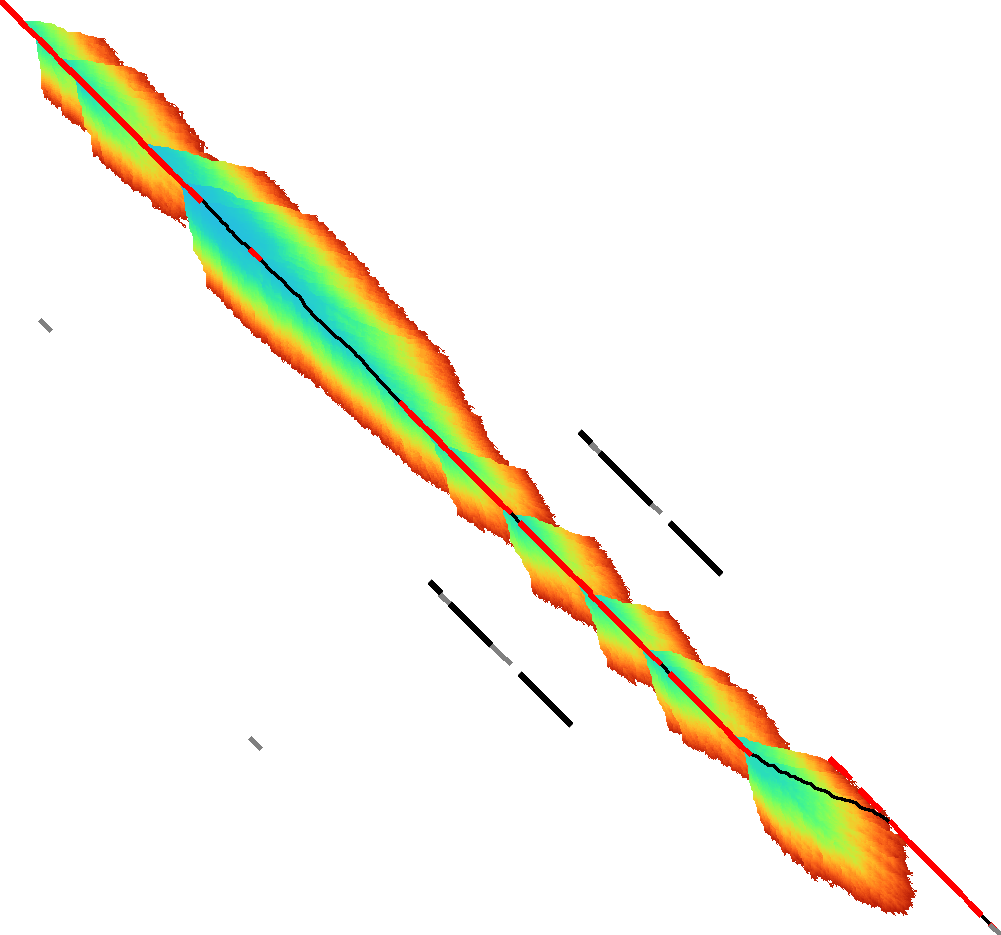
\includegraphics[scale=0.15]{imgs/comparison/sh.png} &
    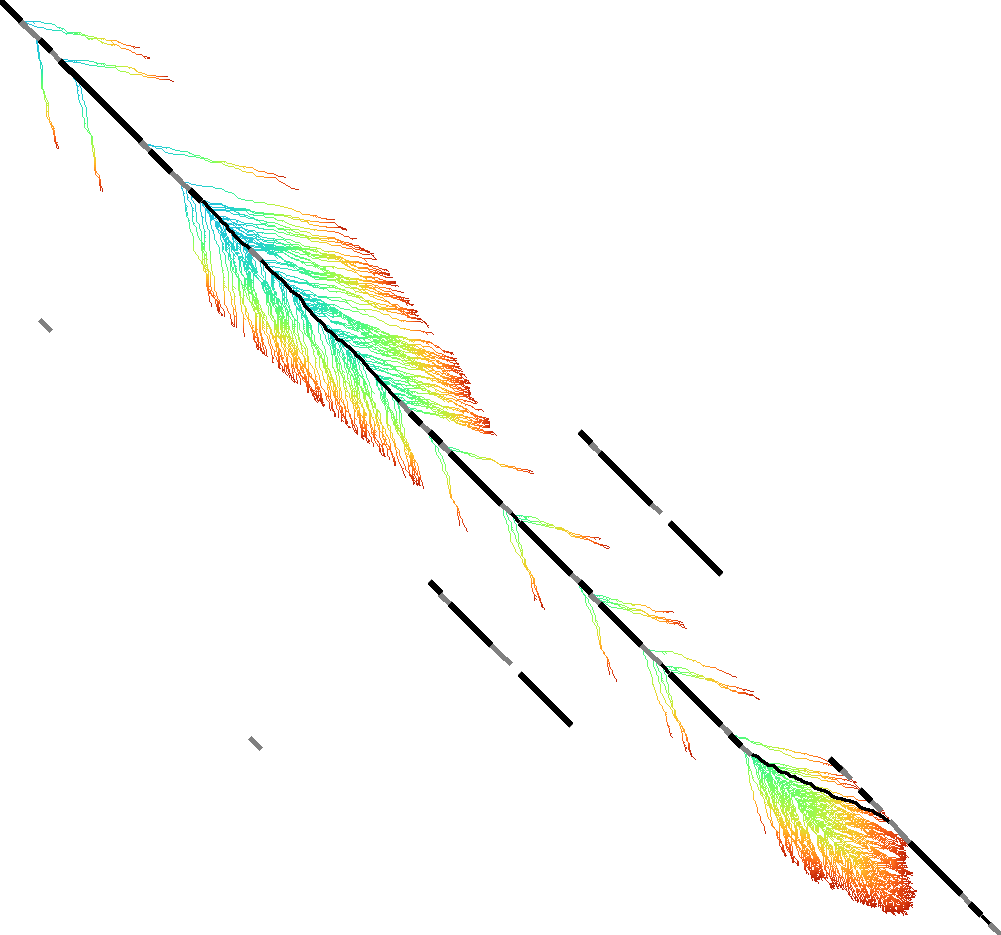
\includegraphics[scale=0.15]{imgs/comparison/sh-noprune-dt.png} &
    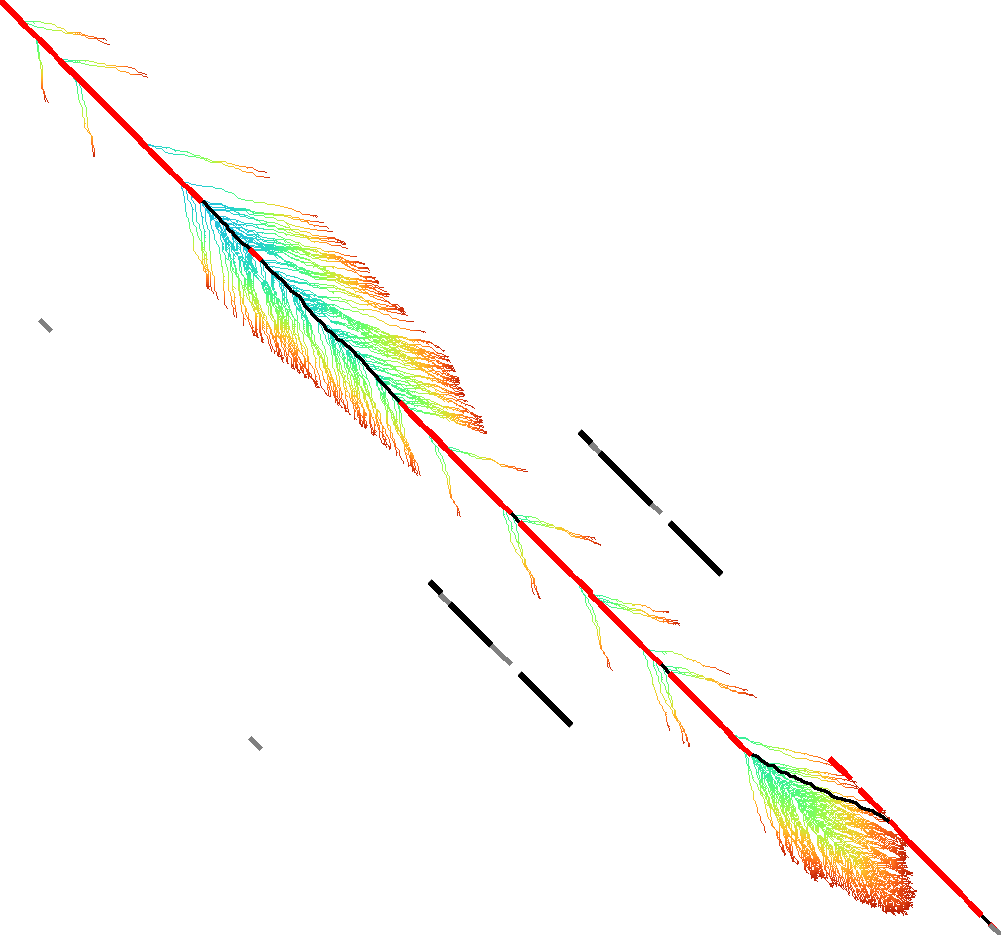
\includegraphics[scale=0.15]{imgs/comparison/sh-dt.png} \\[1cm]
    \textbf{CSH} &
    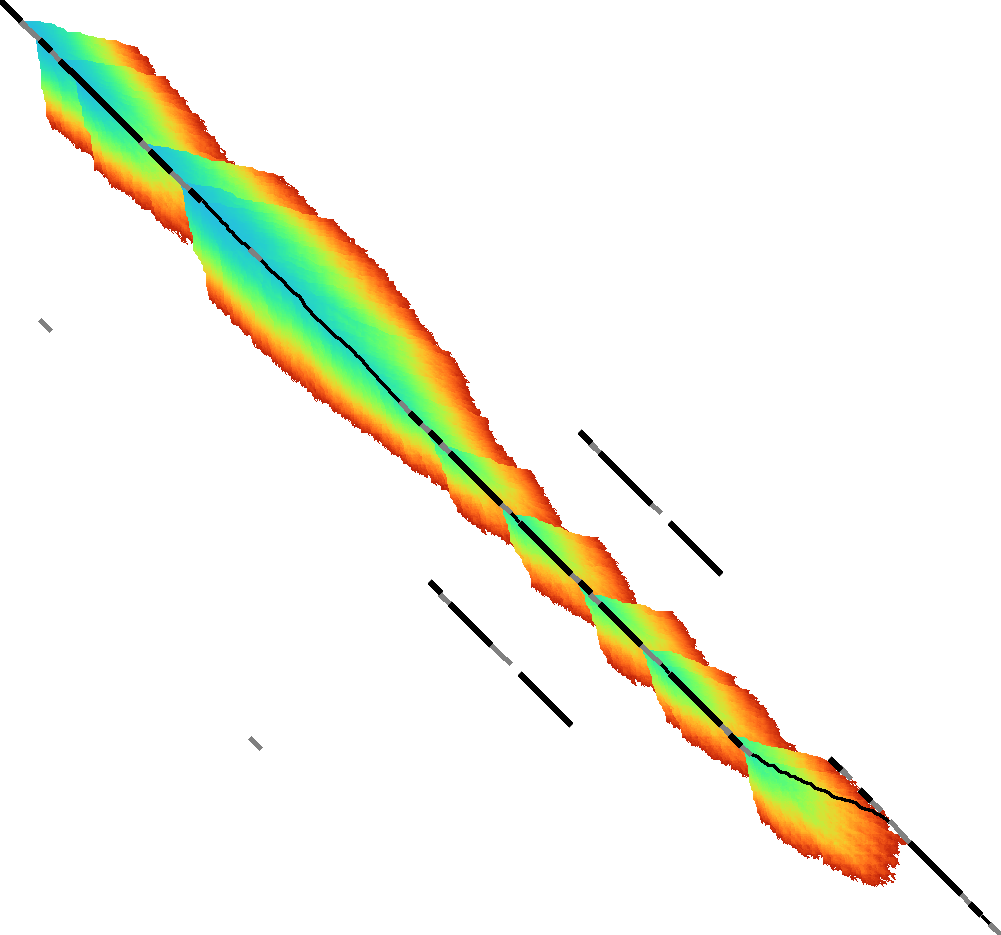
\includegraphics[scale=0.15]{imgs/comparison/csh-noprune.png} &
    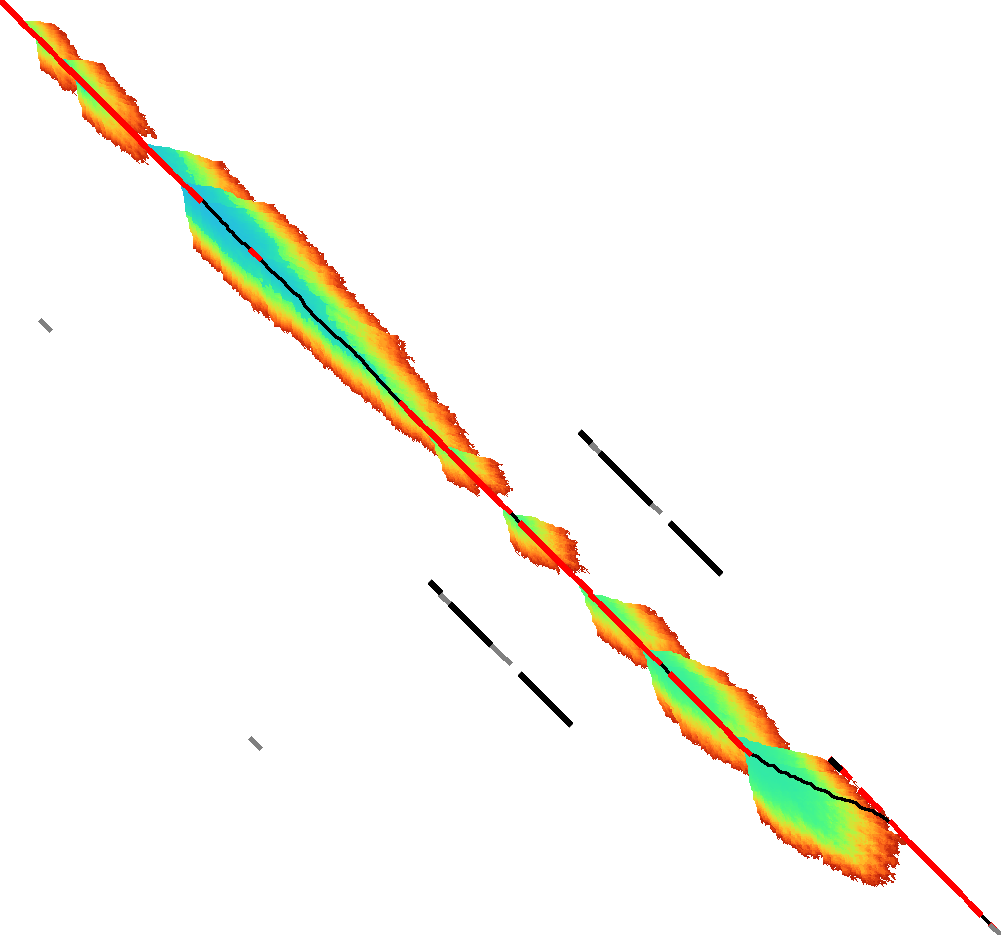
\includegraphics[scale=0.15]{imgs/comparison/csh.png} &
    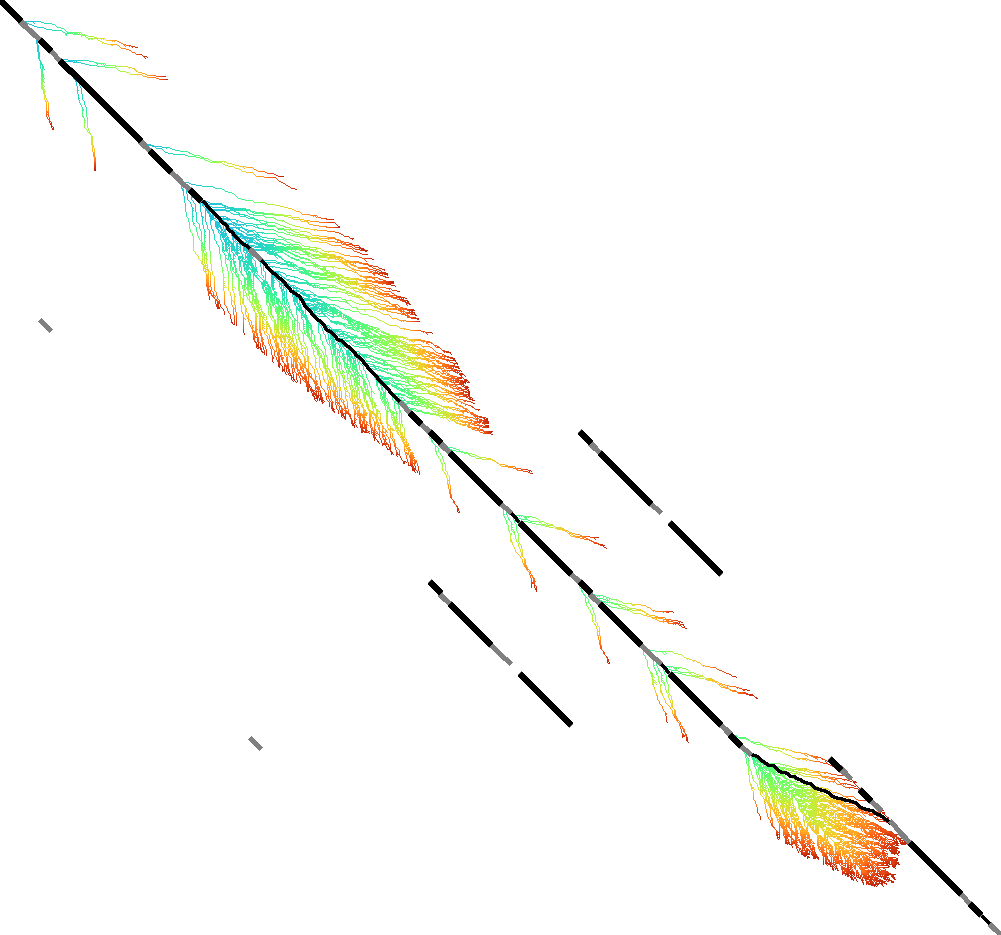
\includegraphics[scale=0.15]{imgs/comparison/csh-noprune-dt.png} &
    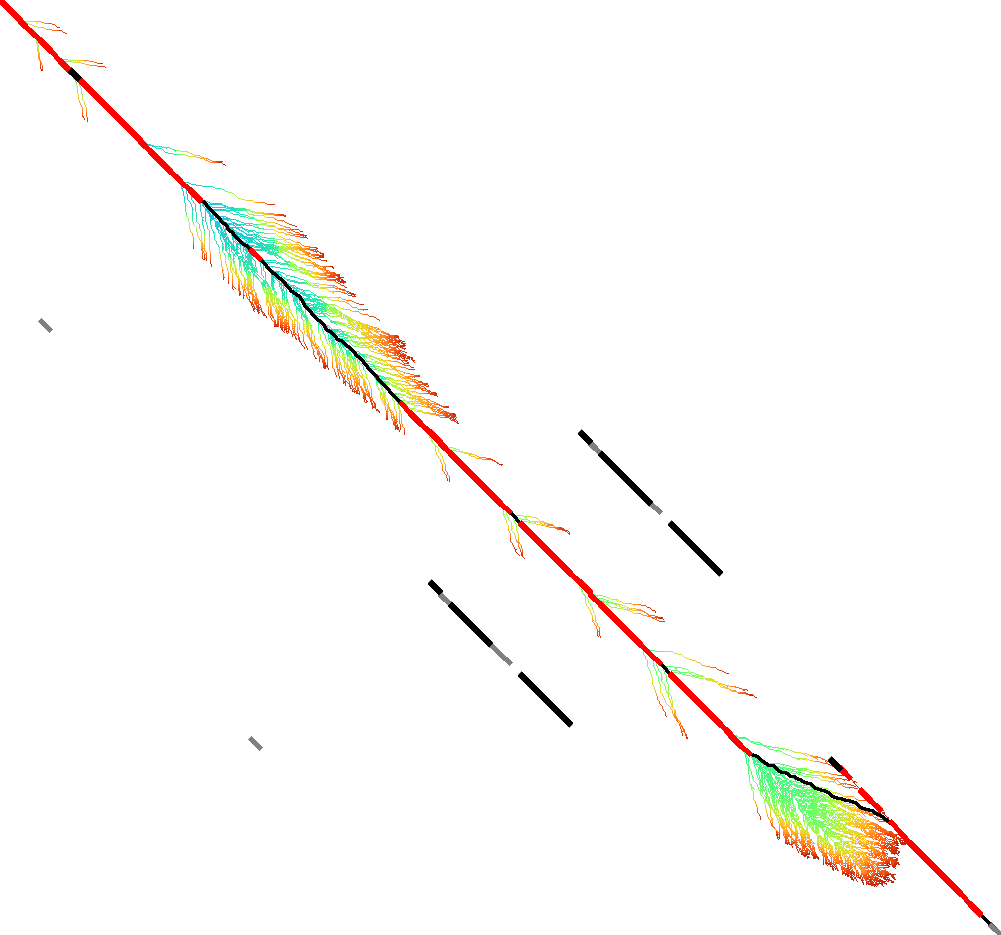
\includegraphics[scale=0.15]{imgs/comparison/csh-dt.png} \\[1cm]
    \textbf{GCSH} &
    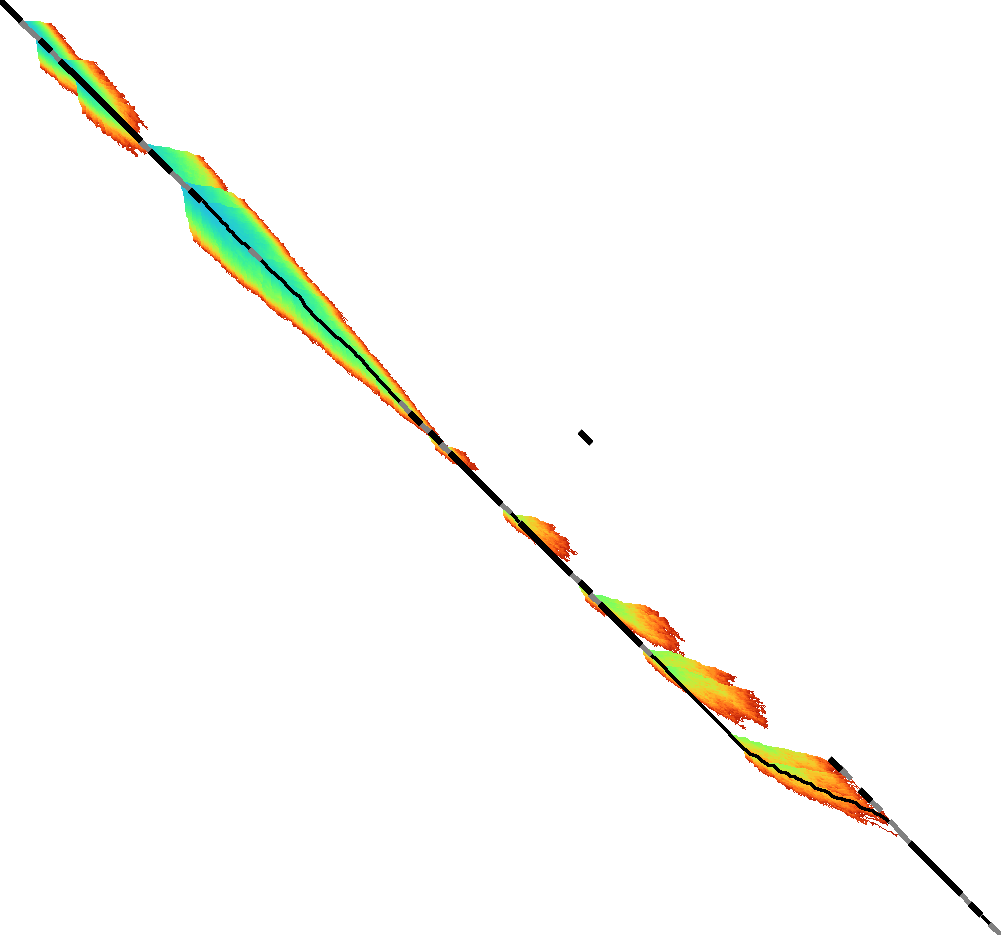
\includegraphics[scale=0.15]{imgs/comparison/gcsh-noprune.png} &
    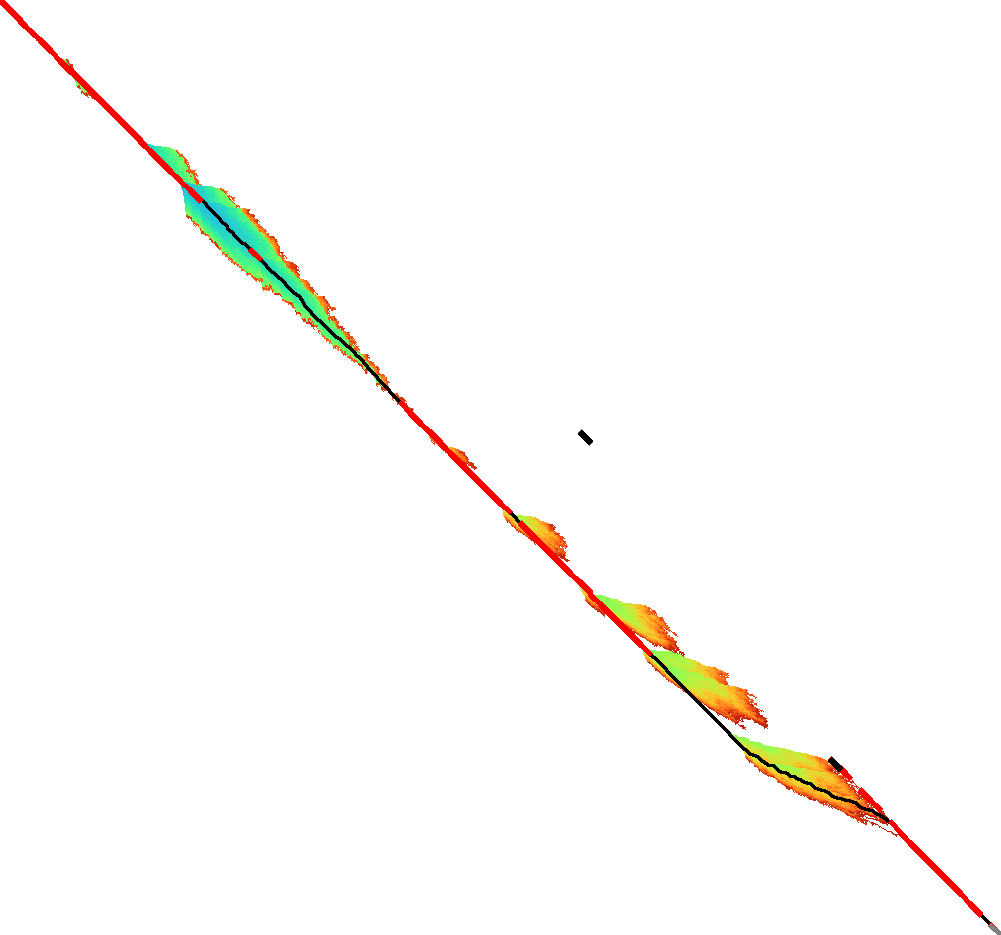
\includegraphics[scale=0.15]{imgs/comparison/gcsh.png} &
    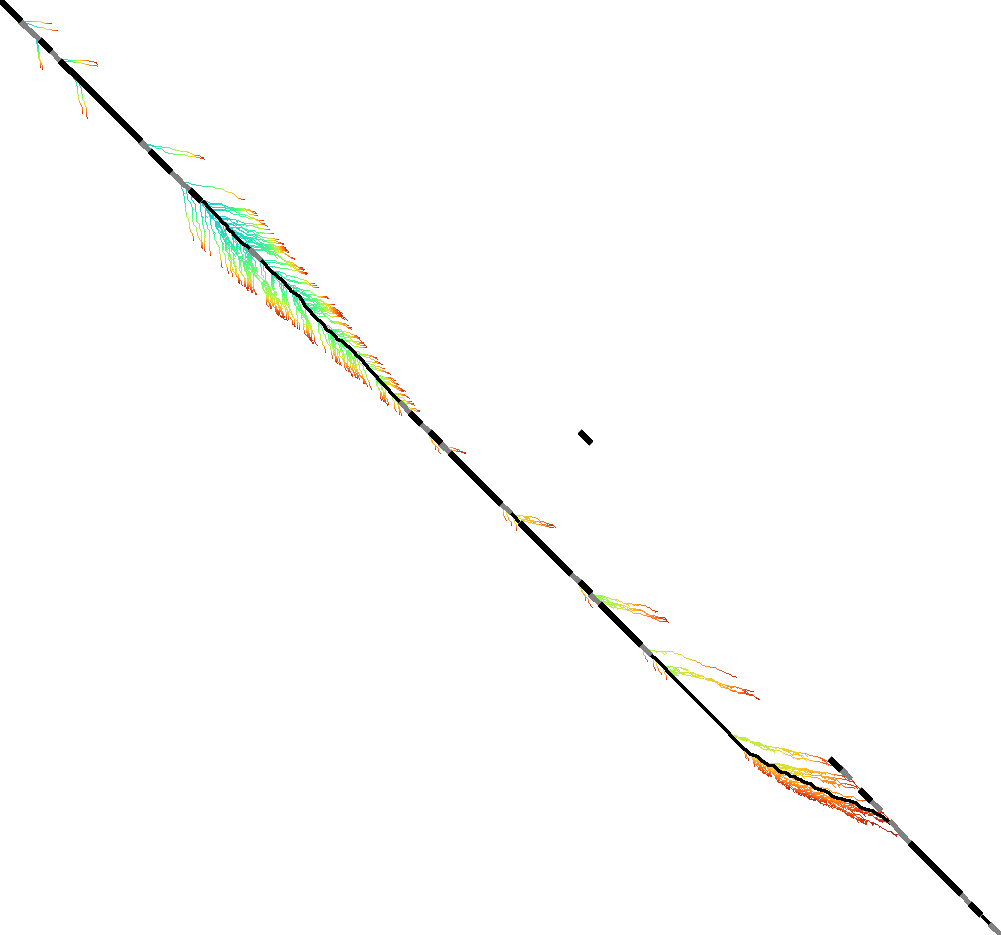
\includegraphics[scale=0.15]{imgs/comparison/gcsh-noprune-dt.png} &
    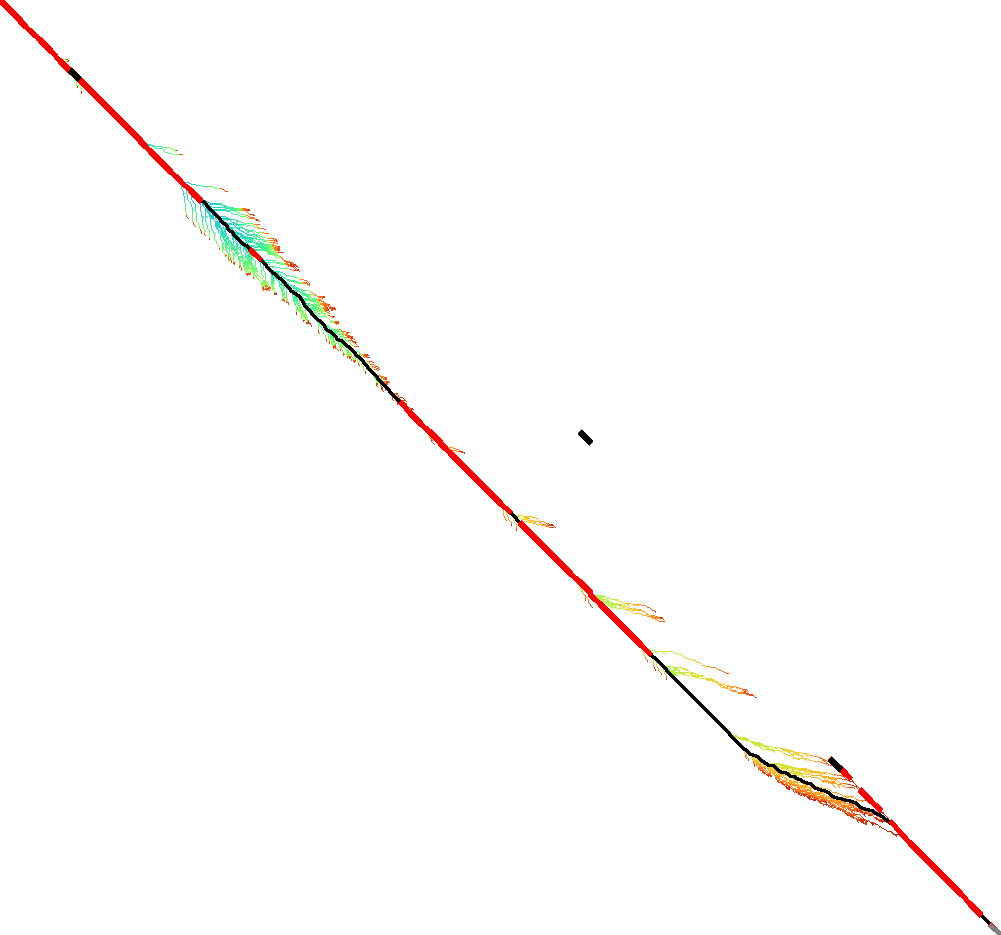
\includegraphics[scale=0.15]{imgs/comparison/gcsh-dt.png} \\
  \end{tabular}
  \caption{\textbf{Expanded states for various heuristics and techniques, on a
      sequence containing a noisy region, a repeat, and an indel} ($n{=}1000$,
      $d{=}17.5\%$). The colour shows the order of expanding, from
      \textcolor{blue}{blue} to \textcolor{red}{red}. The sequences include a
      highly divergent region, a repeat, and a gap. Matches are shown as
      \textbf{black diagonals}, with inexact matches in
      \textbf{\textcolor{gray}{grey}} and pruned matches in
      \textcolor{red}{red}. The final path is \textbf{black}. Dijkstra does not
      have pruning variants, and Dijkstra with DT is equivalent to \oldwfa. More
      accurate heuristics reduce the number of expanded states by more
      effectively punishing repeats (\CSH) and gaps (\GCH). Pruning reduces the
      number of expanded states before the pruned matches, and diagonal
      transition reduces the density of expanded states in quadratic regions.}
  \label{fig:comparison}
\end{figure*}

